% !TeX root = ./Serie05-JoelZuber-YannikDaellenbach.tex
\begin{exercise}
  Erstellen Sie Scribbles für die folgenden vier Seiten einer Kochrezepte-Applikation:
  \begin{itemize}
    \item Login Seite
    \item Profil-Seite des angemeldeten Benutzers
    \item Ansicht aller gesammelten Rezepte
    \item Detailansicht eines Rezeptes
  \end{itemize}
  Erstellen Sie für jede Seite mindestens zwei Varianten.
  \\\\
\end{exercise}

\begin{figure}[H]
  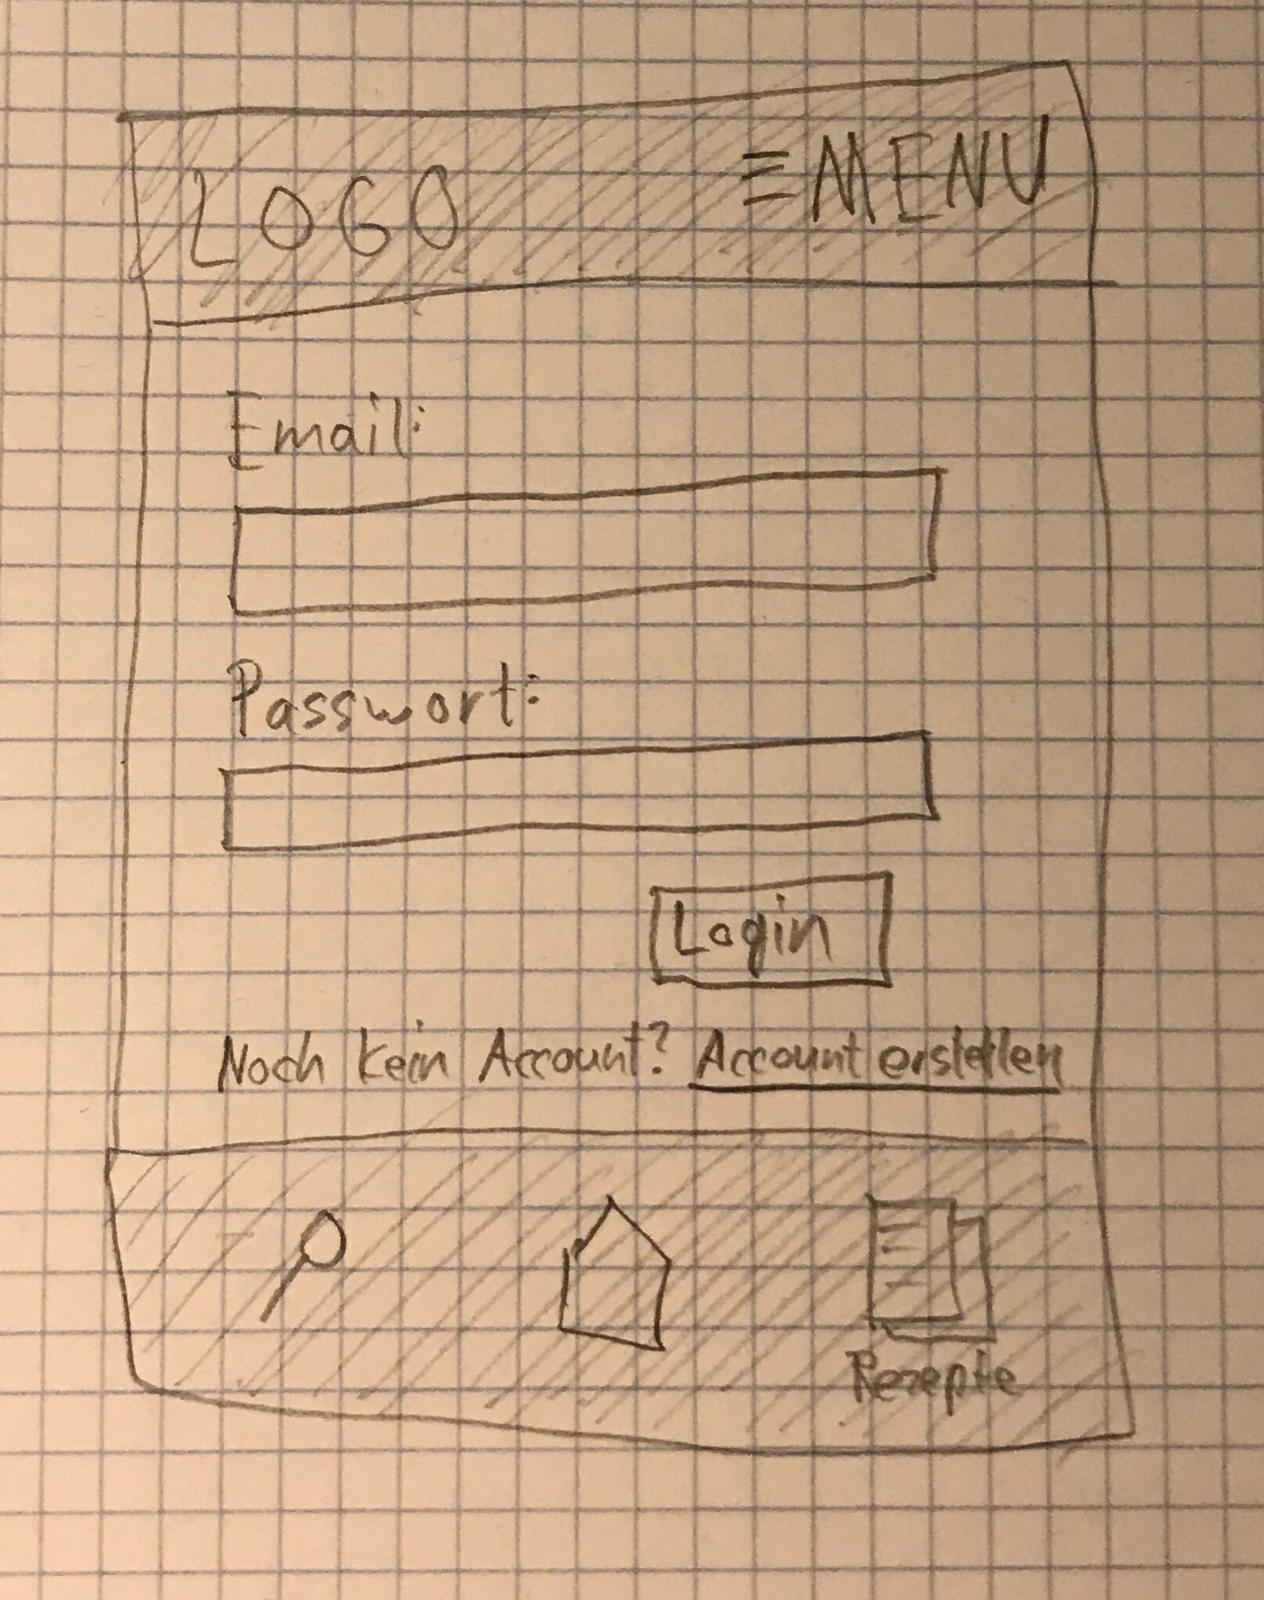
\includegraphics[width=\linewidth]{./exercise13/Login1.jpeg}
  \caption{Login 1}
\end{figure}

\begin{figure}[H]
  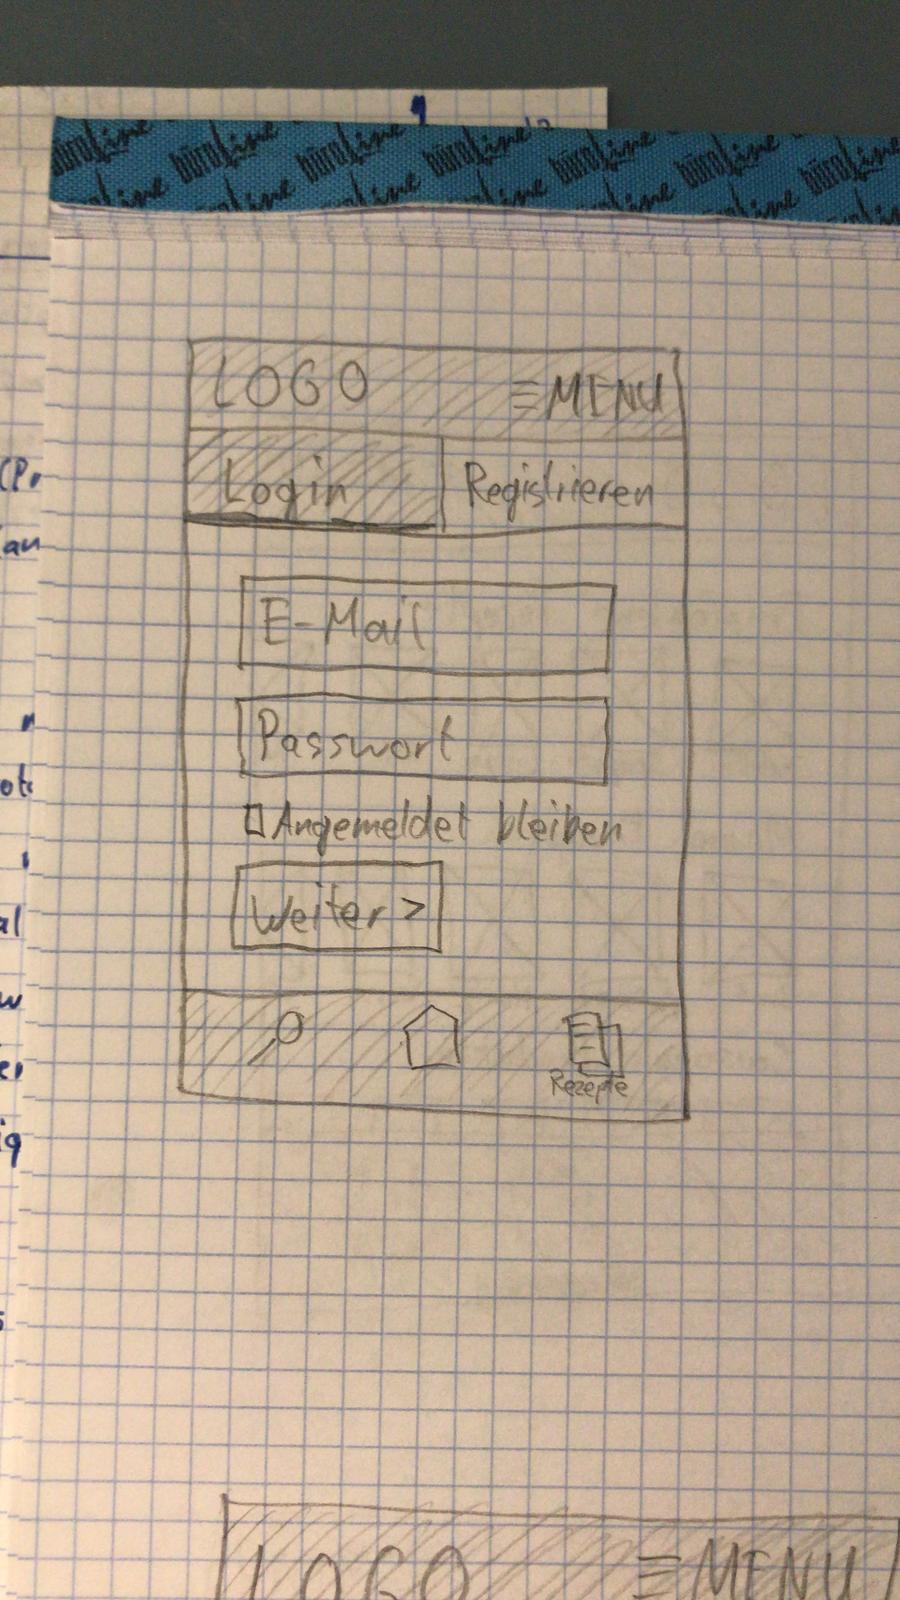
\includegraphics[width=\linewidth]{./exercise13/Login2.jpeg}
  \caption{Login 2}
\end{figure}

\begin{figure}[H]
  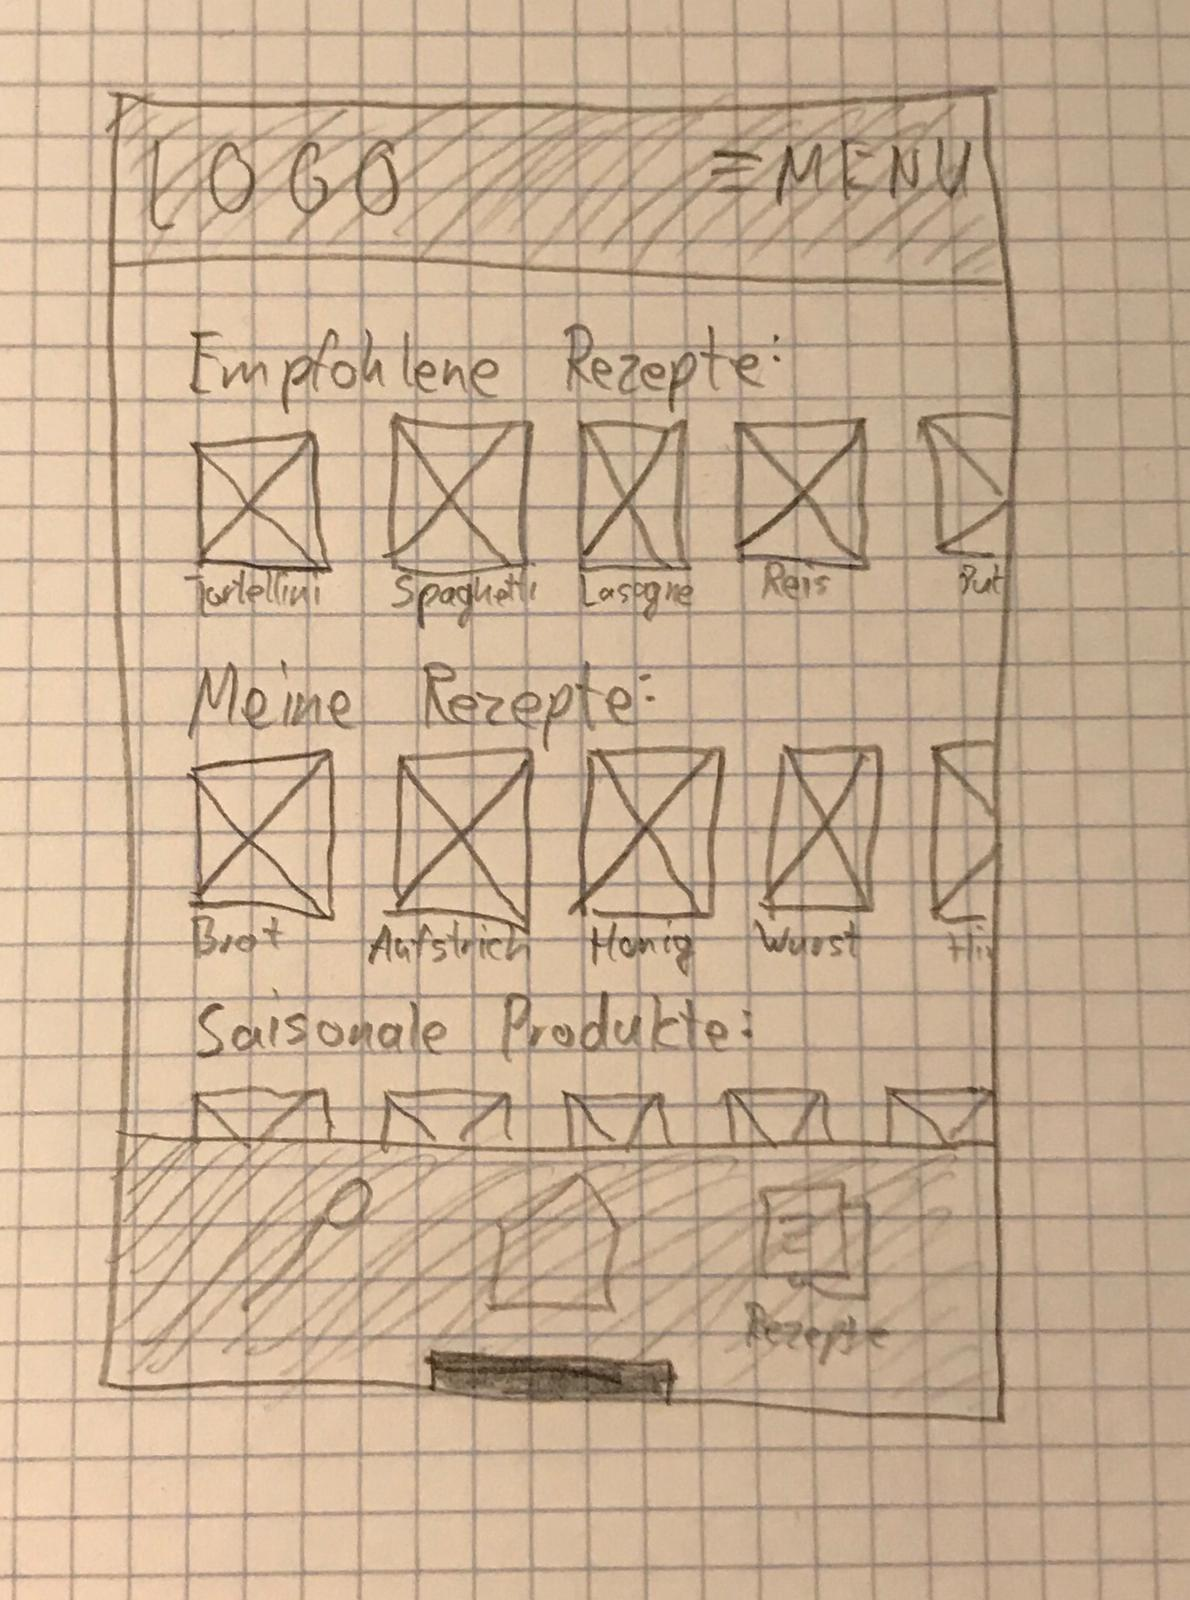
\includegraphics[width=\linewidth]{./exercise13/Profil1.jpeg}
  \caption{Profil 1}
\end{figure}

\begin{figure}[H]
  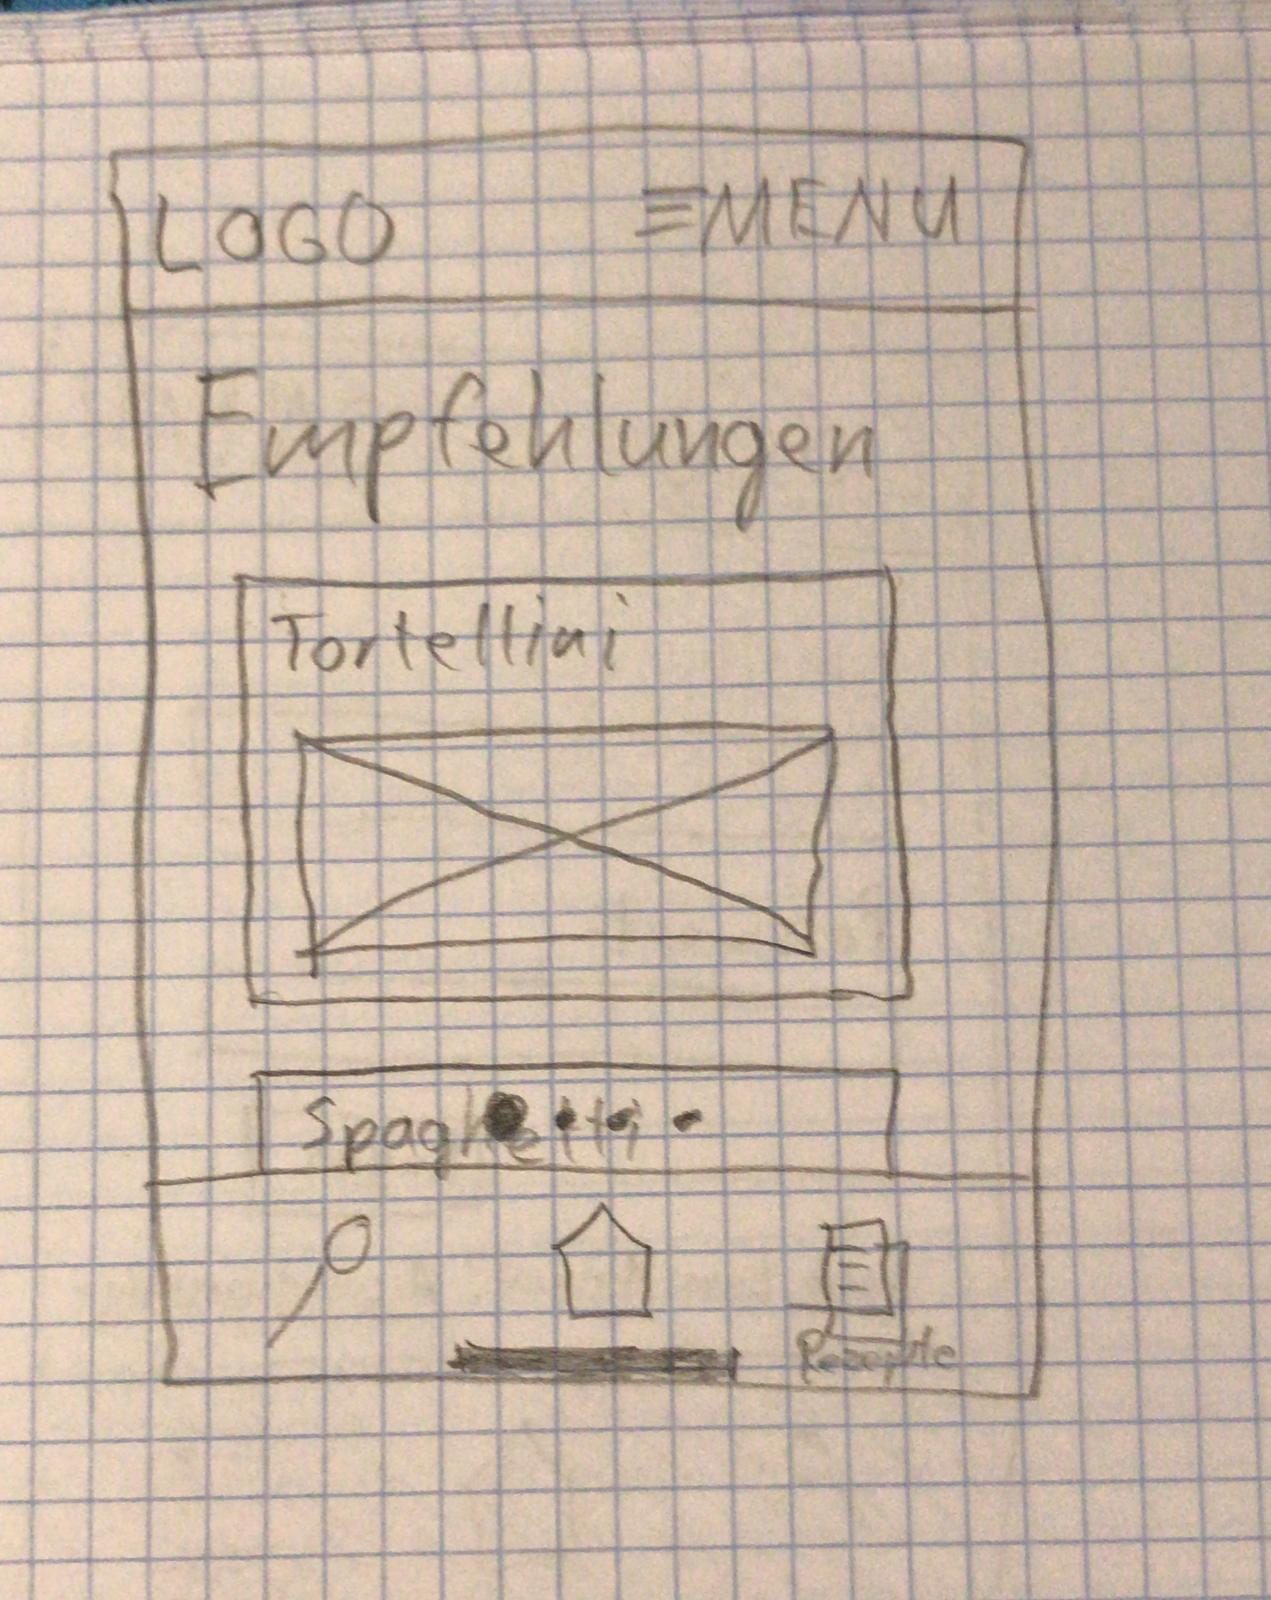
\includegraphics[width=\linewidth]{./exercise13/Profil2.jpeg}
  \caption{Profil 2}
\end{figure}

\begin{figure}[H]
  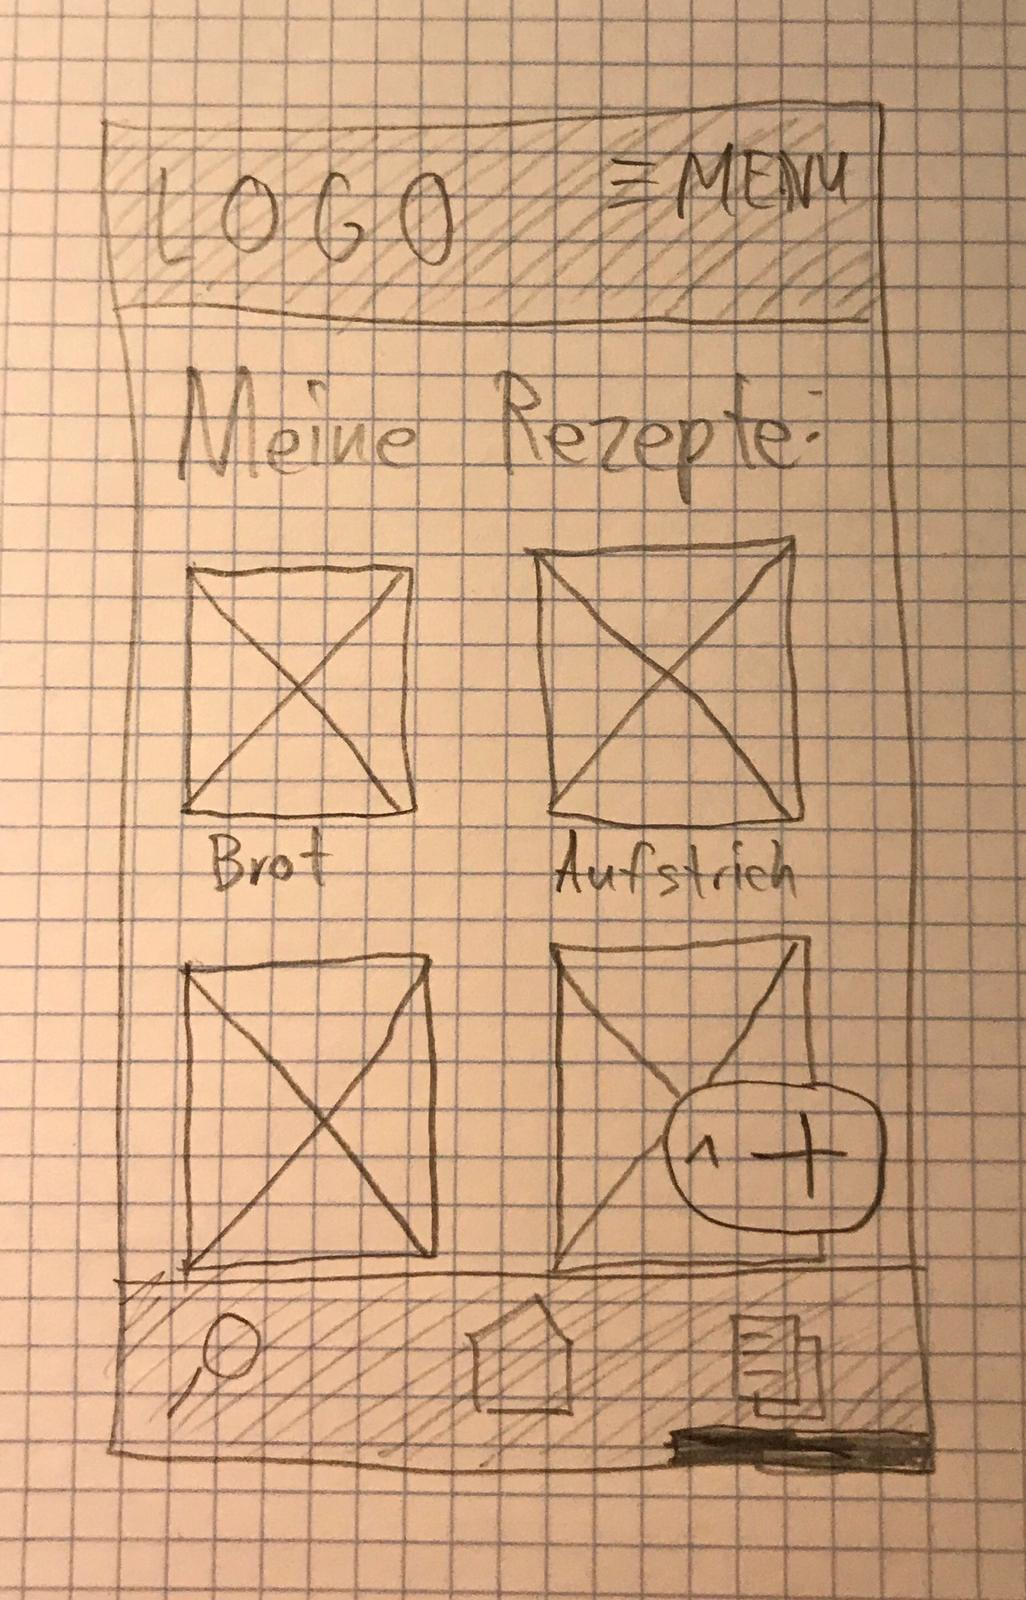
\includegraphics[width=\linewidth]{./exercise13/Rezepte1.jpeg}
  \caption{Rezepte 1}
\end{figure}

\begin{figure}[H]
  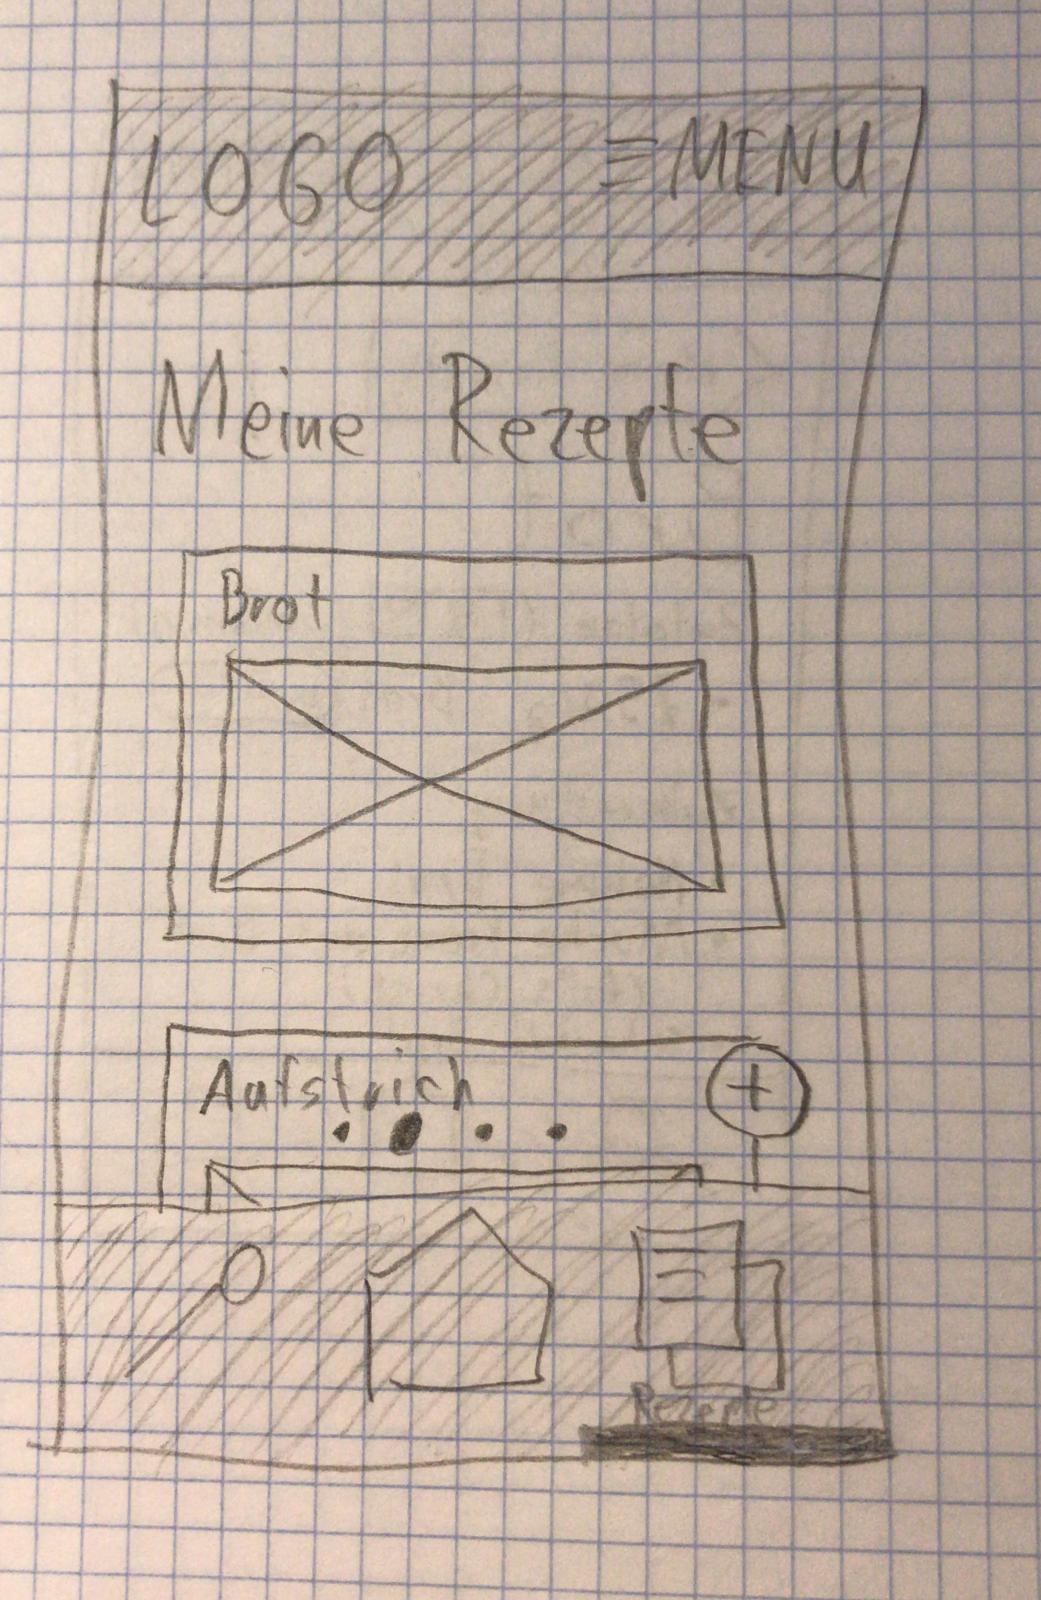
\includegraphics[width=\linewidth]{./exercise13/Rezepte2.jpeg}
  \caption{Rezepte 2}
\end{figure}

\begin{figure}[H]
  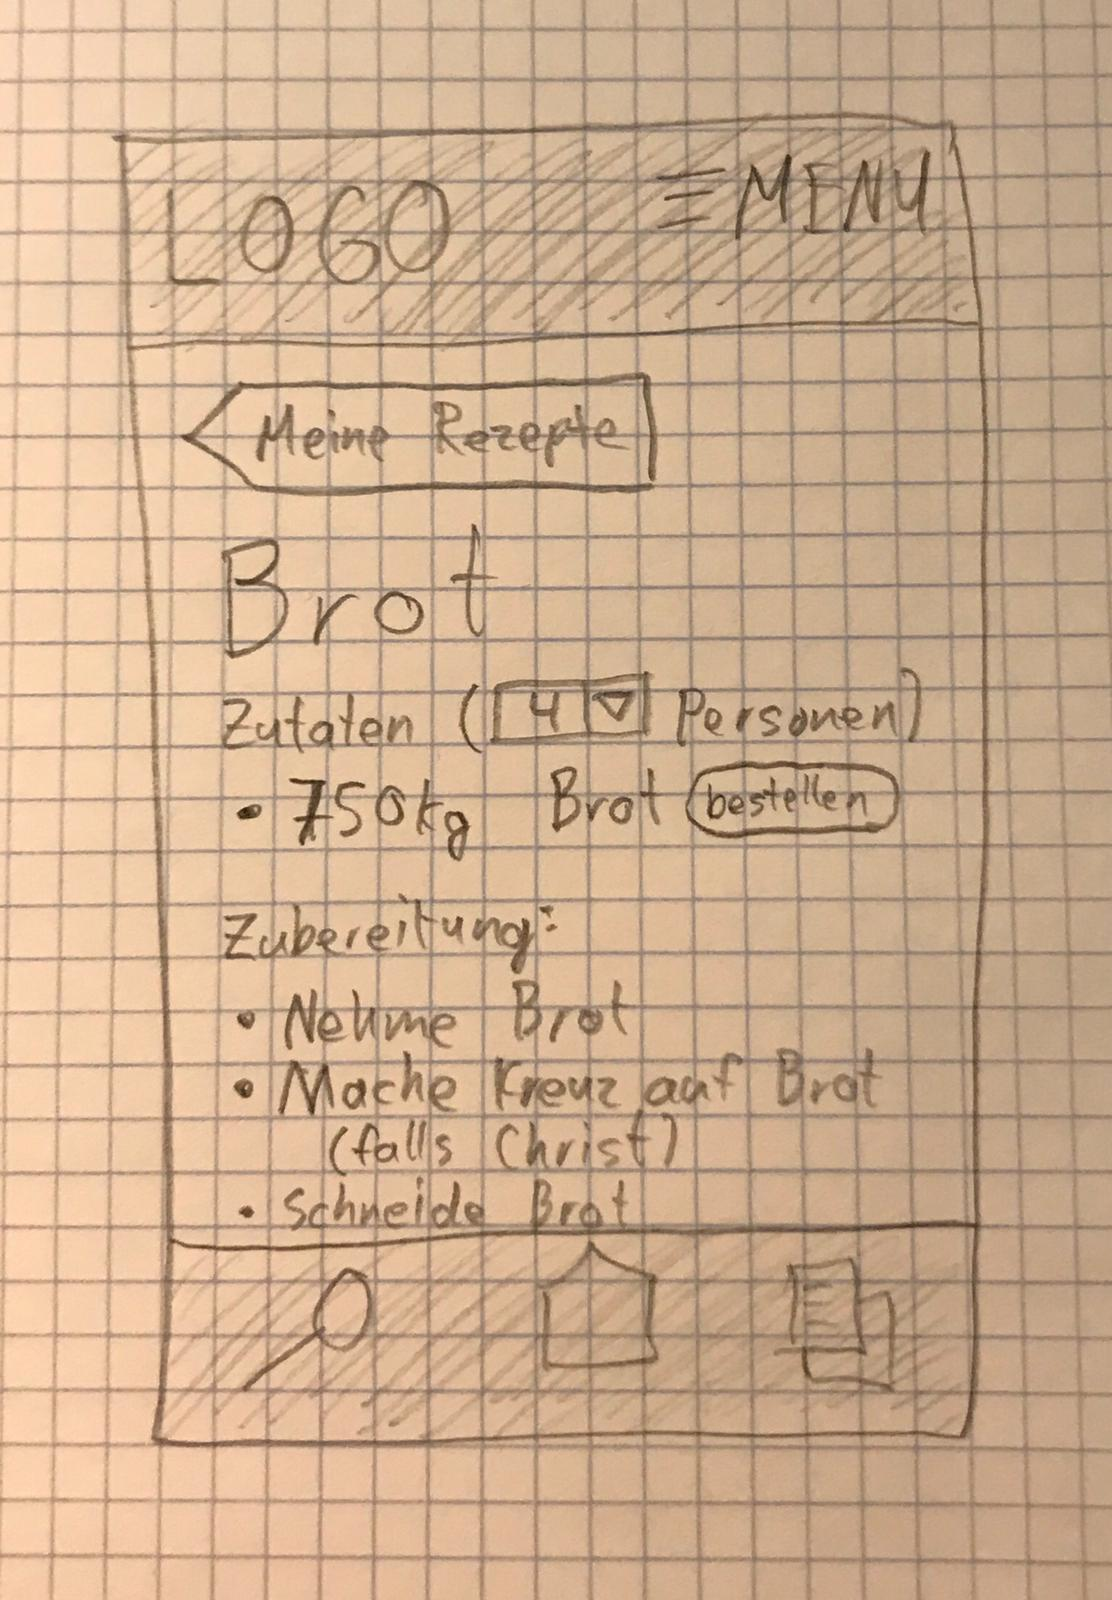
\includegraphics[width=\linewidth]{./exercise13/Detailansicht1.jpeg}
  \caption{Detailansicht 1}
\end{figure}

\begin{figure}[H]
  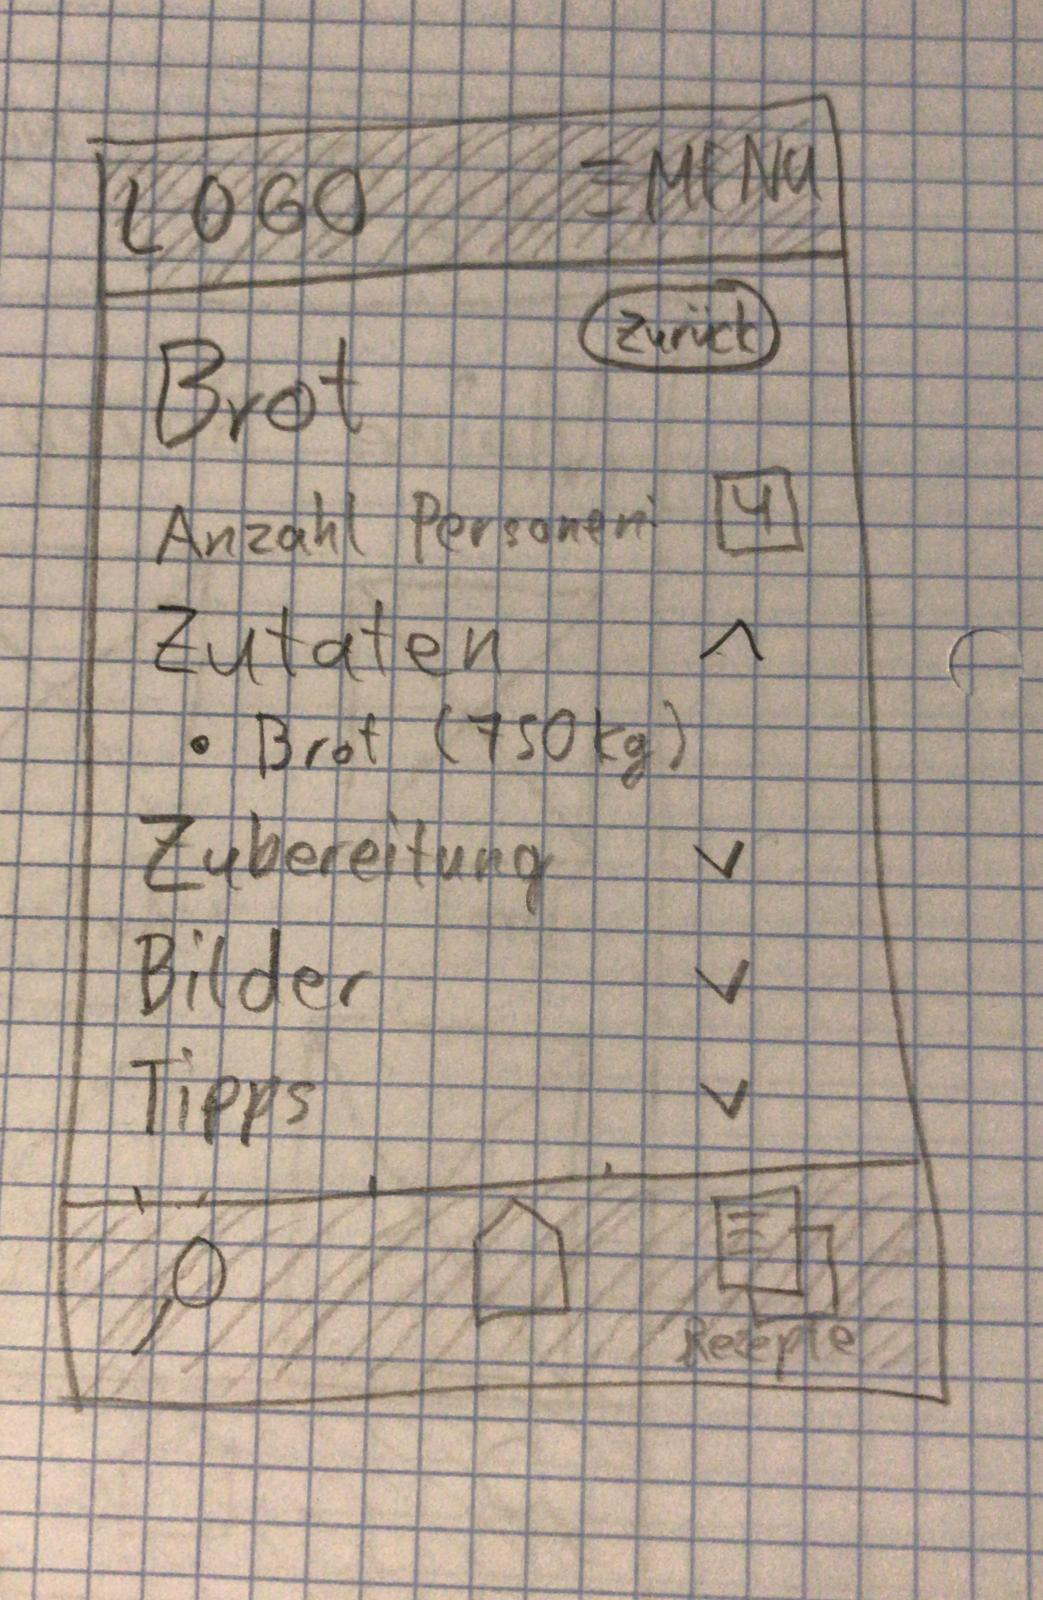
\includegraphics[width=\linewidth]{./exercise13/Detailansicht2.jpeg}
  \caption{Detailansicht 2}
\end{figure}